\vspace*{\fill}
\begin{center}
    {\color{Black} \rule{\linewidth}{1.2mm} }\\
\vspace{0.25in}
    {\centering\fontsize{30}{40}{\bfseries{\color{Black}{\scshape{Chapter IV : }}}}}
\vspace{0.35in}\\
    {\color{Black} \rule{\linewidth}{1.2mm} }
\end{center}
\vspace*{\fill}
\addcontentsline{toc}{chapter}{\color{Black}{Chapter IV : }}
\setcounter{section}{0}

\newpage

\section{Introduction}
\vspace{0.2in}
\hspace*{0.16in}
In this chapter, we will present artificial intelligence with all of its branches, and then dive deeper into convolutional neural networks (CNNs) and their layers. Finally, we will present some CNN architectures and image processing methods.

\section{Artificial Intelligence}
\subsection{Definition}
It is the science and engineering of making intelligent machines, especially intelligent computer programs. It is related to the similar task of using computers to understand human intelligence, but AI does not have to confine itself to methods that are biologically observable. \textsuperscript{\cite{mccarthy2004artificial}}

\vspace{0.2in}

\begin{figure}[h]
\centering
  \vspace{-0.1in}
    \centerline{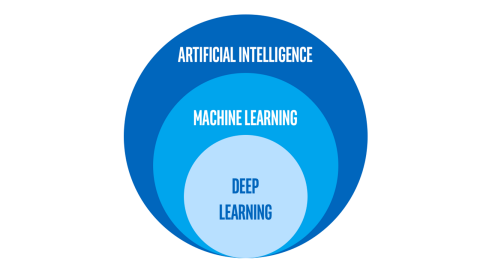
\includegraphics[width = 4in, height = 2.2in]{../images/artificial-intelligence.png}}
    \caption{Artificial Intelligence}
\end{figure}

Artificial intelligence algorithms can be categorised into these four main types:

\begin{itemize}
    \item \textbf{Supervised learning:}
        Supervised learning, as the name indicates, has the presence of a supervisor as a teacher. Basically supervised learning is when we teach or train the machine using data that is well labeled. Which means some data is already tagged with the correct answer. After that, the machine is provided with a new set of examples (data) so that the supervised learning algorithm analyses the training data (set of training examples) and produces a correct outcome from labeled data. \textsuperscript{\cite{AITypes-GeeksForGeeks}}

    \item \textbf{Unsupervised learning:}
        Unsupervised learning is the training of a machine using information that is neither classified nor labeled and allowing the algorithm to act on that information without guidance. Here the task of the machine is to group unsorted information according to similarities, patterns, and differences without any prior training of data. \textsuperscript{\cite{AITypes-GeeksForGeeks}}

    \vspace{0.2in}

    \begin{table}[H]
\centering
\resizebox{\textwidth}{!}{%
\begin{tabular}{|
>{\columncolor[HTML]{FFFFFF}}c |
>{\columncolor[HTML]{FFFFFF}}c |
>{\columncolor[HTML]{FFFFFF}}c 
>{\columncolor[HTML]{FFFFFF}}l 
>{\columncolor[HTML]{FFFFFF}}l |}
\hline
\textbf{Parameters}               & \textbf{Supervised machine learning} & \multicolumn{3}{c|}{\cellcolor[HTML]{FFFFFF}\textbf{Unsupervised machine learning}} \\ \hline
\textbf{Input Data} &
  \begin{tabular}[c]{@{}c@{}}Algorithms are trained\\ using labeled data.\end{tabular} &
  \multicolumn{3}{c|}{\cellcolor[HTML]{FFFFFF}\begin{tabular}[c]{@{}c@{}}Algorithms are used against\\ data that is not labeled\end{tabular}} \\ \hline
\textbf{Computational Complexity} & Simpler method                       & \multicolumn{3}{c|}{\cellcolor[HTML]{FFFFFF}Computationally complex}                \\ \hline
\textbf{Accuracy}                 & Highly accurate                      & \multicolumn{3}{c|}{\cellcolor[HTML]{FFFFFF}Less accurate}                          \\ \hline
\end{tabular}%
}
\caption{Table that presents diffrence between supervised and unsupervised machine learning \textsuperscript{\cite{AITypes-GeeksForGeeks}}}
\label{Table that presents diffrence between supervised and unsupervised machine learning}
\end{table}


    \item \textbf{Semi Supervised learning:}
        Semi-supervised learning sits somewhere between Supervised and Unsupervised learning algorithms. It employs a mix of labeled and unlabeled datasets. It works with data that has only a few labels; it usually works with unlabeled data. Labels are expensive, yet for corporate purposes, a few labels may suffice.
    \item \textbf{Reinforcement learning:}
        Reinforcement learning is just a machine learning approach that rewards positive behavior while penalizing poor behavior. In general, a reinforcement learning agent is capable of sensing and interpreting its environment, acting, and learning via trial and error. Developers of reinforcement learning propose a way of rewarding desired behaviors and punishing negative behaviors. \textsuperscript{\cite{SSLvsRL-askanydifference}}

    \vspace{0.2in}

    \begin{table}[H]
\centering
\resizebox{\textwidth}{!}{%
\begin{tabular}{|c|c|cll|}
\hline
\rowcolor[HTML]{FFFFFF} 
\textbf{Parameters}               & \textbf{Semi-Supervised Learning} & \multicolumn{3}{c|}{\cellcolor[HTML]{FFFFFF}\textbf{Reinforcement Learning}} \\ \hline
\rowcolor[HTML]{FFFFFF} 
\textbf{Definition} &
  \begin{tabular}[c]{@{}c@{}}Uses a small amount of labeled\\ data bolstering a larger\\ set of unlabeled data\end{tabular} &
  \multicolumn{3}{c|}{\cellcolor[HTML]{FFFFFF}An algorithm witha reward system} \\ \hline
\rowcolor[HTML]{FFFFFF} 
\textbf{Aim} &
  \begin{tabular}[c]{@{}c@{}}To counter the disadvantages of\\ supervised and unsupervised\\ learning.\end{tabular} &
  \multicolumn{3}{c|}{\cellcolor[HTML]{FFFFFF}\begin{tabular}[c]{@{}c@{}}To learn a series\\ of action\end{tabular}} \\ \hline
\rowcolor[HTML]{FFFFFF} 
\textbf{Interaction of the agent} & Doesn’t interact                  & \multicolumn{3}{c|}{\cellcolor[HTML]{FFFFFF}Interacts}                       \\ \hline
\textbf{Practical application} &
  \begin{tabular}[c]{@{}c@{}}Speech analysis, internet\\ content classification\end{tabular} &
  \multicolumn{3}{c|}{\begin{tabular}[c]{@{}c@{}}Trajectory optimization, motion\\ planning\end{tabular}} \\ \hline
\textbf{Labels}                   & It has labels.                    & \multicolumn{3}{c|}{It doesn’t have labels.}                                 \\ \hline
\end{tabular}%
}
\caption{Comparison Table Between Semi-Supervised and Reinforcement Learning \textsuperscript{\cite{SSLvsRL-askanydifference}}}
\label{Comparison Table Between Semi-Supervised and Reinforcement Learning}
\end{table}

\end{itemize}

\subsection{Machine Learning}
Machine learning is a branch of artificial intelligence (AI) and computer science which focuses on the use of data and algorithms to imitate the way that humans learn, gradually improving its accuracy. \textsuperscript{\cite{ML-IBM}}

\begin{itemize}
  \item \textbf{Linear Regression:}
      Linear Regression is a machine learning algorithm based on supervised learning. It performs a regression task. Regression models a target prediction value based on independent variables. It is mostly used for finding out the relationship between variables and forecasting. Different regression models differ based on – the kind of relationship between dependent and independent variables they are considering, and the number of independent variables getting used. \textsuperscript{\cite{LR-GeeksForGeeks}}
  \item \textbf{Support Vector Machines:}
      Support Vector Machine (SVM) is a computer algorithm that learns by example to assign labels to objects. \textsuperscript{\cite{boser1992training}} For instance, an SVM can learn to recognize fraudulent credit card activity by examining hundreds or thousands of fraudulent and nonfraudulent credit card activity reports. Alternatively, an SVM can learn to recognize handwritten digits by examining a large collection of scanned images of handwritten zeroes, ones and so fourth. \textsuperscript{\cite{noble2006support}}
  \item \textbf{Gradient Descent:}
      Gradient descent is an optimization algorithm used to minimize some function by iteratively moving in the direction of steepest descent as defined by the negative of the gradient. In machine learning, we use gradient descent to update the parameters of our model. Parameters refer to coefficients in Linear Regression and weights in neural networks. \textsuperscript{\cite{DG-ml-cheatsheet}}
\end{itemize}

\subsection{Deep Learning}
\subsubsection{Neural Networks}
Artificial neural networks (ANNs) are comprised of a node layers, containing an input layer, one or more hidden layers, and an output layer. Each node, or artificial neuron, connects to another and has an associated weight and threshold. If the output of any individual node is above the specified threshold value, that node is activated, sending data to the next layer of the network. Otherwise, no data is passed along to the next layer of the network.


\begin{figure}[H]
\centering
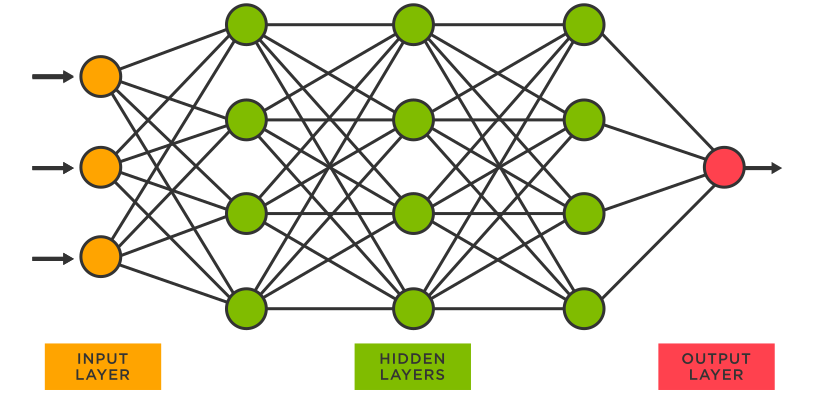
\includegraphics[width=\linewidth]{../images/neural-network-diagram.png}
\caption{Architecture of Neural Network}
\label{fig:NN}
\end{figure}

Neural networks rely on training data to learn and improve their accuracy over time. However, once these learning algorithms are fine-tuned for accuracy, they are powerful tools in computer science and artificial intelligence, allowing us to classify and cluster data at a high velocity. Tasks in speech recognition or image recognition can take minutes versus hours when compared to the manual identification by human experts. One of the most well-known neural networks is Google’s search algorithm.

if we dive into the details, we can consider that each node has it's linear regression model, composed of input data, weights, a bias (or threshold), and an output. The formula would look something like equation \ref{eq:NN-Node-Activation}:

%\begin{figure}[H]
%\centering
%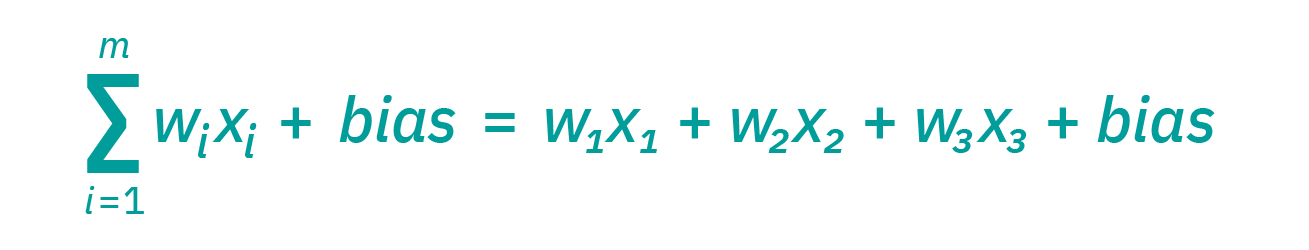
\includegraphics[width=\linewidth]{../images/NN-Node-equation.png}
%\caption{Architecture of Neural Network}
%\label{fig:NN}
%\end{figure}

\begin{equation}
    \sum_{i=1}^{m} W_{i}X_{i} + bias = W_{1}X_{1} + W_{2}X_{2} + W_{3}X_{3} + bias
    \label{eq:NN-Node-Activation}
\end{equation}

\begin{equation}
    output = f(x) = 
    \begin{cases}
        1 & if \sum_{i=1}^{m} W_{1}X_{1} + b \leq 0 \\
        0 & if \sum_{i=1}^{m} W_{1}X_{1} + b < 0
    \end{cases}
    \label{eq:NN-Node-Activation2}
\end{equation}

Once an input layer is determined, weights are assigned. These weights help determine the importance of any given variable, with larger ones contributing more significantly to the output compared to other inputs. All inputs are then multiplied by their respective weights and then summed (similar to eaquation \ref{eq:NN-Node-Activation}). Afterward, the output is passed through an activation function as we can see in equation \ref{eq:NN-Node-Activation2}, which determines the output. If that output exceeds a given threshold, it “fires” (or activates) the node, passing data to the next layer in the network. This results in the output of one node becoming in the input of the next node. This process of passing data from one layer to the next layer defines this neural network as a feedforward network.

\subsubsection{Convolutional Neural Networks}
CNNs or ConvNets are among the most successful and widely used architectures in the deep learning community, especially for computer vision tasks. CNNs were initially proposed by Fukushima in his seminal paper on the “Neocognitron” \textsuperscript{\cite{fukushima_Neocognitron}}.

\begin{figure}[H]
\centering
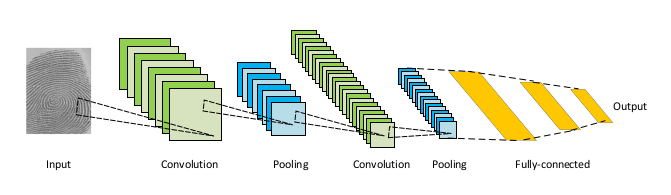
\includegraphics[width=\linewidth]{../images/CNN.png}
\caption{Architecture of convolutional neural networks. From \textsuperscript{\cite{minaee2021image}}}
\label{fig:CNN}
\end{figure}

Convolutional neural networks are distinguished from other neural networks by their superior performance with image, speech, or audio signal inputs. They have three main types of layers, which are:

\begin{itemize}
    \item Convolutional layer
    \item Pooling layer
    \item Fully-connected (FC) layer
\end{itemize}

The convolutional layer is the first layer of a convolutional network. While convolutional layers can chained by additional convolutional layers or pooling layers, the fully-connected layer is the final layer. With each layer, the CNN increases in its complexity, identifying greater portions of the image. Earlier layers focus on simple features, such as colors and edges. As the image data progresses through the layers of the CNN, it starts to recognize larger elements or shapes of the object until it finally identifies the intended object. 
    
    
\begin{enumerate}
    \item \textbf{Convolutional layer} : \\
        The convolutional layer is the core building block of a CNN, and it is where the majority of computation occurs. It requires a few components, which are input data, a filter, and will output a feature map. Let’s assume that the input will be a color image, which is made up of a matrix of pixels in 3D. This means that the input will have three dimensions—a height, width, and depth—which correspond to RGB in an image. We also have a feature detector, also known as a kernel or a filter, which will move across the receptive fields of the image, checking if the feature is present. This process is known as a convolution. \textsuperscript{\cite{CNN-IBM}} \\
        The feature detector is a two-dimensional (2-D) array of weights, which represents part of the image. While they can vary in size, the filter size is typically a 3x3 matrix; this also determines the size of the receptive field. The filter is then applied to an area of the image, and a dot product is calculated between the input pixels and the filter. This dot product is then fed into an output array. Afterwards, the filter shifts by a stride, repeating the process until the kernel has swept across the entire image. The final output from the series of dot products from the input and the filter is known as a feature map, activation map, or a convolved feature.
        \begin{figure}[H]
            \centering
            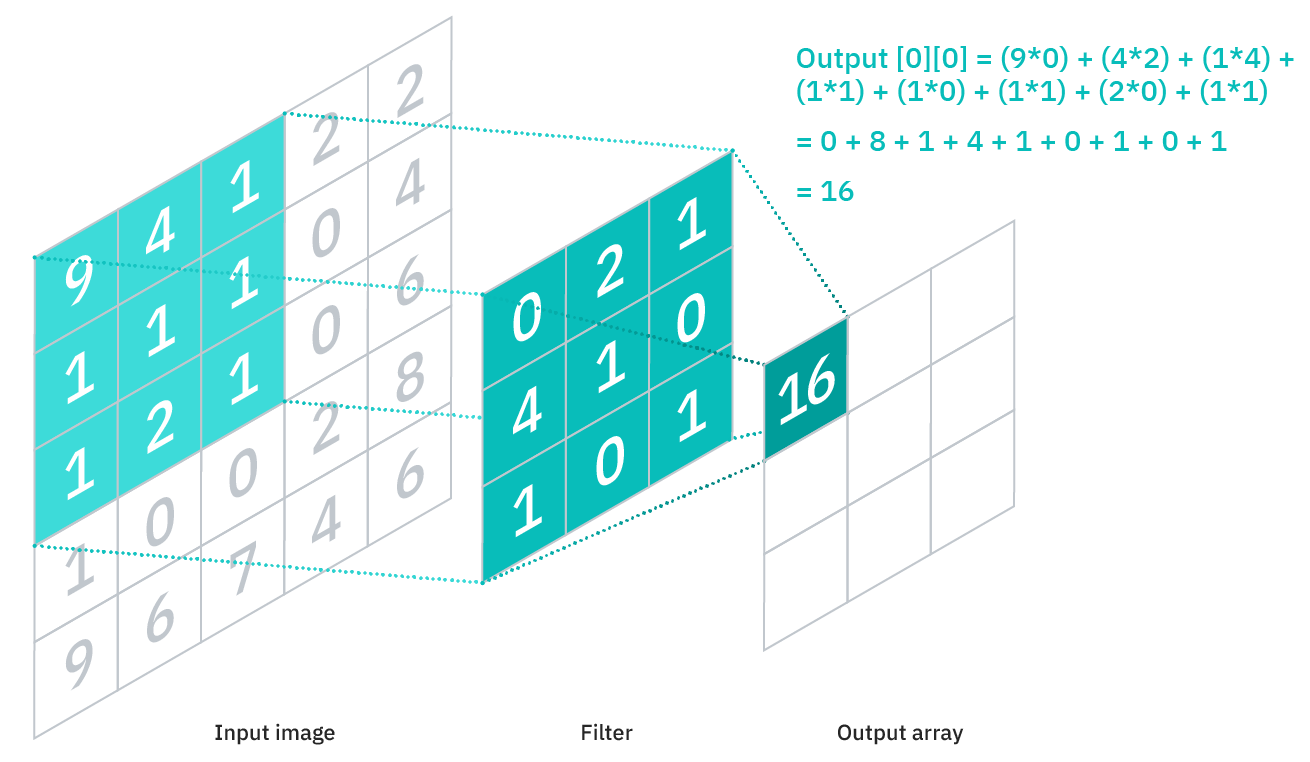
\includegraphics[width=10cm]{../images/CNN-kernel.png}
            \caption{CNN kernel}
            \label{fig:CNN-kernel}
        \end{figure}
        as we can see in the fig \ref{fig:CNN-kernel}, the kernel will browse all the matrix by shifting it's position. where the weights in the kernel will remain fixed as it moves across the image, which is also known as parameter sharing. Some parameters, like the weight values, adjust during training through the process of backpropagation and gradient descent. However, there are three hyperparameters which affect the volume size of the output that need to be set before the training of the neural network begins. These include:
        \begin{itemize}
            \item \textbf{The number of filters} affects the depth of the output. For example, three distinct filters will give us three different feature maps, creating a depth of three.
            \item \textbf{Stride} is the distance, or number of pixels, that the kernel moves over the input matrix. While stride values of two or greater is rare, a larger stride yields a smaller output.
            \item \textbf{Zero-padding }is usually used when the filters do not fit the input image. This sets all elements that fall outside of the input matrix to zero, producing a larger or equally sized output. There are three types of padding:
            \begin{itemize}
                \item \textbf{Valid padding}: This is also known as no padding. In this case, the last convolution is dropped if dimensions do not align.
                \item \textbf{Same padding}: This padding ensures that the output layer has the same size as the input layer
                \item \textbf{Full padding}: This type of padding increases the size of the output by adding zeros to the border of the input.
            \end{itemize}
        \end{itemize}
        
        \begin{figure}[H]
            \centering
            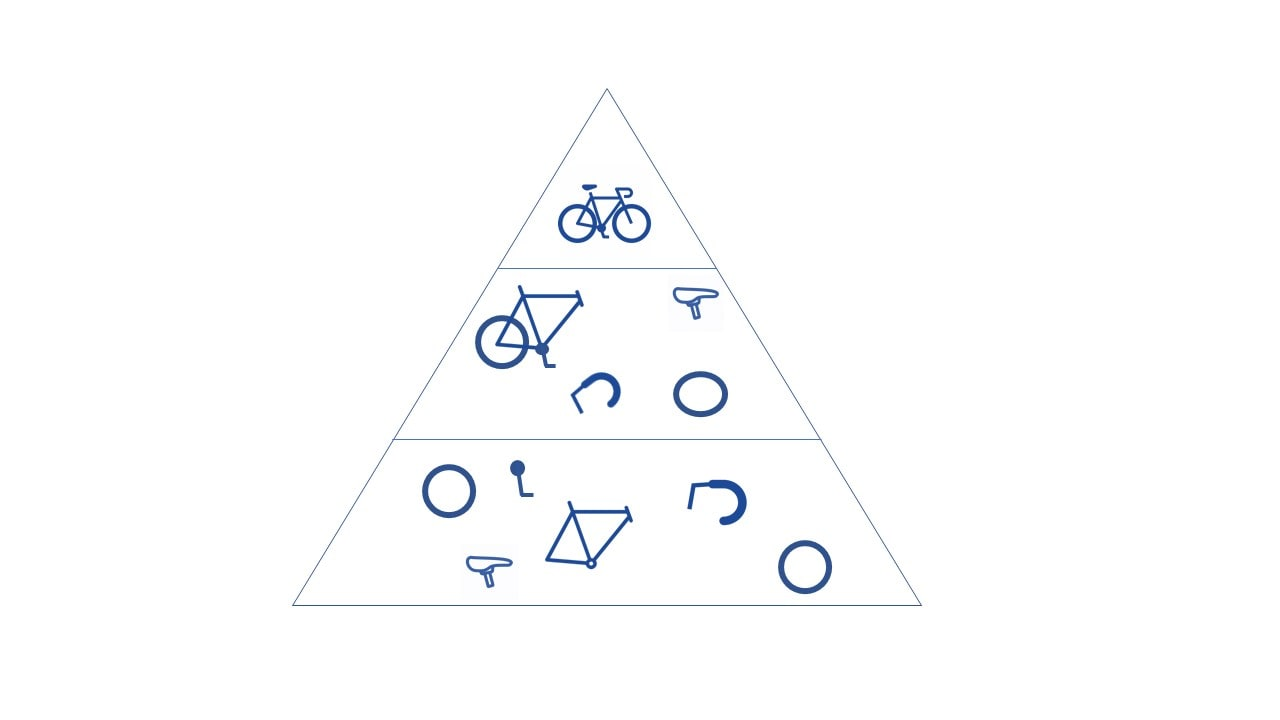
\includegraphics[width=10cm]{../images/CNN-Feature-Hierarchy.jpg}
            \caption{Feature Hierarchy}
            \label{fig:CNN-Feature-Hierarchy}
        \end{figure}
        
        After each convolution operation, a CNN applies an activation function to the feature map, the most used activation function is the Rectified Linear Unit (ReLU).\\
        As we mentioned earlier, when we chain convolutional layers, the structure of the CNN can become hierarchical as the later layers can see the pixels within the receptive fields of prior layers.  As an example, let’s assume that we’re trying to determine if an image contains a bicycle. You can think of the bicycle as a sum of parts. It is comprised of a frame, handlebars, wheels, pedals, et cetera. Each individual part of the bicycle makes up a lower-level pattern in the neural net, and the combination of its parts represents a higher-level pattern, creating a feature hierarchy within the CNN.
    \item \textbf{Pooling Layer}:\\
        Pooling layers, also known as downsampling, conducts dimensionality reduction, reducing the number of parameters in the input. Similar to the convolutional layer, the pooling operation sweeps a filter across the entire input, but the difference is that this filter does not have any weights. Instead, the kernel applies an aggregation function to the values within the receptive field, populating the output array. There are two main types of pooling:
        \begin{itemize}
            \item \textbf{Max pooling}: As the filter moves across the input, it selects the pixel with the maximum value to send to the output array. As an aside, this approach tends to be used more often compared to average pooling.
            \item \textbf{Average pooling}: As the filter moves across the input, it calculates the average value within the receptive field to send to the output array.
        \end{itemize}
        
        While a lot of information is lost in the pooling layer, it also has a number of benefits to the CNN. They help to reduce complexity, improve efficiency, and limit risk of overfitting.
    
    \item \textbf{Fully-Connected Layer}:\\
        The name of the fully-connected layer aptly describes itself. The pixel values of the input image are not directly connected to the output layer in partially connected layers. However, in the fully-connected layer, each node in the output layer connects directly to a node in the previous layer.

        This layer performs the task of classification based on the features extracted through the previous layers and their different filters. While convolutional and pooling layers tend to use ReLu functions or other activation functions, FC layers usually leverage a softmax or sigmoid activation function to classify inputs appropriately, producing a probability from 0 to 1.
        
\end{enumerate}


\section{CNN architectures}
\vspace{0.2in}
\hspace*{0.16in}

In this section we are going to present some CNN architectures, CNN architectures are preDesigned models targeting a spcial task like image segmentation, feature extraction, classification ..., all the architectures can be an encoder or decoder and it can be both.
\begin{itemize}
    \item \textbf{encoder:} also called contracting path which consist of the downsampling of the feature map by using multiple convolutional and max pooling layers and it differs between model architectures.
    \item \textbf{decoder:} also called expansive path wich consist of an upsampling of the feature map by using up-convolution (which concatenates the feature map from the upper parallel encoder layers)
\end{itemize}

\begin{figure}[h]
    \centering
      \vspace{-0.1in}
        \centerline{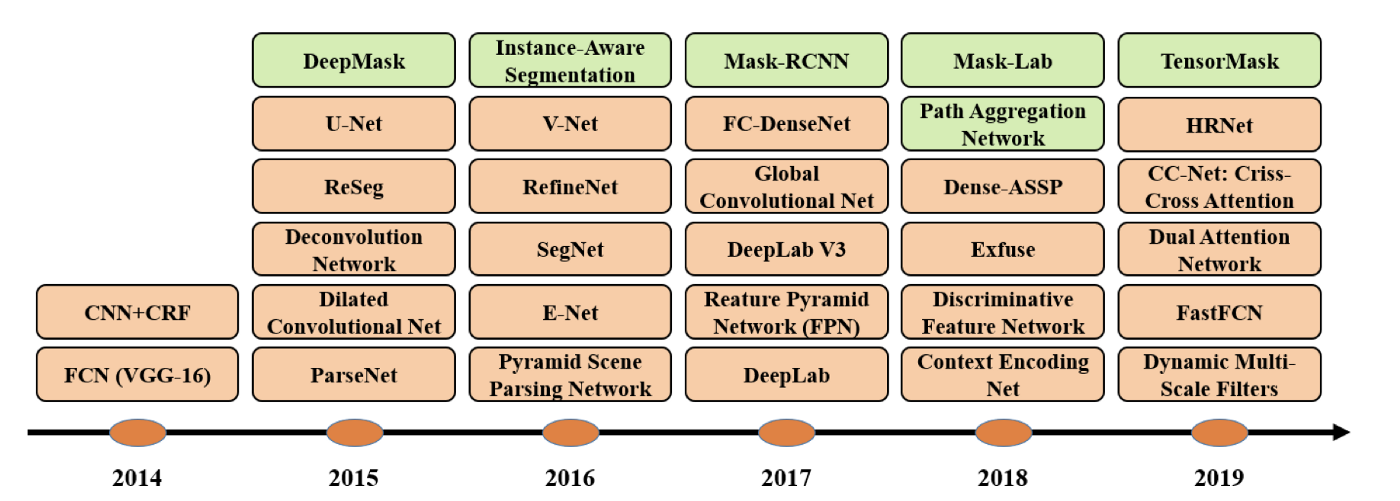
\includegraphics[width = 6in, height = 2.2in]{../images/timeline-of-segmentation-algorithms.png}}
        \caption{Timeline of segmentation algorithms}
    \end{figure}


\subsection{VGG}
VGG stands for Visual Geometry Group; it is a standard deep Convolutional Neural Network (CNN) architecture with multiple layers. The “deep” refers to the number of layers with VGG-16 or VGG-19 consisting of 16 and 19 convolutional layers.\\

The VGG architecture is the basis of ground-breaking object recognition models. Developed as a deep neural network, the VGGNet also surpasses baselines on many tasks and datasets beyond ImageNet. Moreover, it is now still one of the most popular image recognition architectures. 

\subsubsection{VGG16}
The VGG model, or VGGNet, that supports 16 layers is also referred to as VGG16, which is a convolutional neural network model proposed by A. Zisserman and K. Simonyan from the University of Oxford in 2014. These researchers published their model in the research paper titled, “Very Deep Convolutional Networks for Large-Scale Image Recognition.” \textsuperscript{\cite{simonyan2014very}} 

The VGG16 model achieves almost 92.7\% top-5 test accuracy in ImageNet. ImageNet is a dataset consisting of more than 14 million images belonging to nearly 1000 classes. Moreover, it was one of the most popular models submitted to ILSVRC-2014. It replaces the large kernel-sized filters with several 3×3 kernel-sized filters one after the other, thereby making significant improvements over AlexNet. The VGG16 model was trained using Nvidia Titan Black GPUs for multiple weeks.

As mentioned above, the VGGNet-16 supports 16 layers and can classify images into 1000 object categories, including keyboard, animals, pencil, mouse, etc. Additionally, the model has an image input size of 224-by-224.

\subsubsection{VGG19}
The concept of the VGG19 model (also VGGNet-19) is the same as the VGG16 except that it supports 19 layers. The “16” and “19” stand for the number of weight layers in the model (convolutional layers). This means that VGG19 has three more convolutional layers than VGG16. 

\subsubsection{VGG Architecture}
VGGNets are based on the most essential features of convolutional neural networks (CNN).
The VGG network is constructed with very small convolutional filters. The VGG-16 consists of 13 convolutional layers and three fully connected layers.
To sum it all up, VGG architecture consists of:

\begin{itemize}
    \item \textbf{Input:} The VGGNet takes in an image input size of 224×224. For the ImageNet competition, the creators of the model cropped out the center 224×224 patch in each image to keep the input size of the image consistent.
    \item \textbf{Convolutional Layers:} VGG’s convolutional layers leverage a minimal receptive field, i.e., 3×3, the smallest possible size that still captures up/down and left/right. Moreover, there are also 1×1 convolution filters acting as a linear transformation of the input. This is followed by a ReLU unit, which is a huge innovation from AlexNet that reduces training time. ReLU stands for rectified linear unit activation function; it is a piecewise linear function that will output the input if positive; otherwise, the output is zero. The convolution stride is fixed at 1 pixel to keep the spatial resolution preserved after convolution (stride is the number of pixel shifts over the input matrix).
    \item \textbf{Hidden Layers:} All the hidden layers in the VGG network use ReLU. VGG does not usually leverage Local Response Normalization (LRN) as it increases memory consumption and training time. Moreover, it makes no improvements to overall accuracy.
    \item \textbf{Fully-Connected Layers:} The VGGNet has three fully connected layers. Out of the three layers, the first two have 4096 channels each, and the third has 1000 channels, 1 for each class.
\end{itemize}

\subsubsection{VGG16 architecture}
The number 16 in the name VGG refers to the fact that it is 16 layers deep neural network (VGGnet). This means that VGG16 is a pretty extensive network and has a total of around 138 million parameters. Even according to modern standards, it is a huge network. However, VGGNet16 architecture’s simplicity is what makes the network more appealing. Just by looking at its architecture, it can be said that it is quite uniform.

There are a few convolution layers followed by a pooling layer that reduces the height and the width. If we look at the number of filters that we can use, around 64 filters are available that we can double to about 128 and then to 256 filters. In the last layers, we can use 512 filters.

\begin{figure}[h]
\centering
    \centerline{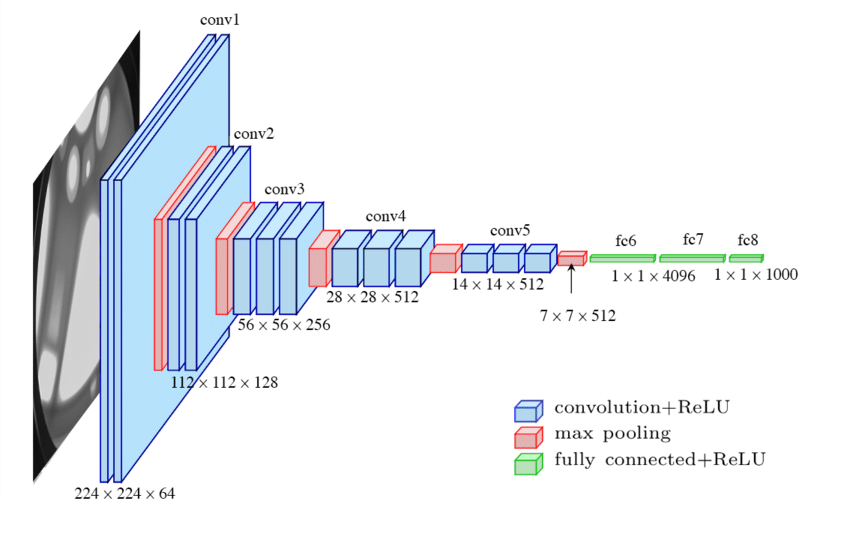
\includegraphics[width = 4.2in, height = 2.4in]{../images/VGG16-architecture.png}}
    \caption{VGG16 architecture}
\end{figure}

\subsubsection{Performance of VGG Models}
VGG16 highly surpasses the previous versions of models in the ILSVRC-2012 and ILSVRC-2013 competitions. Moreover, the VGG16 result is competing for the classification task winner (GoogLeNet with 6.7\% error) and considerably outperforms the ILSVRC-2013 winning submission Clarifai. It obtained 11.2\% with external training data and around 11.7\% without it. In terms of the single-net performance, the VGGNet-16 model achieves the best result with about 7.0\% test error, thereby surpassing a single GoogLeNet by around 0.9\%. \textsuperscript{\cite{VGG-Gaudenz_Boesch}}

\subsection{U-Net}
U-Net is a CNN architecture built for biomedical image segmentation in 2015 \textsuperscript{\cite{ronneberger2015u}}. It consists of a contracting path (encoder) and an expansive path (decoder). The encoder follows the typical architecture of a convolutional network. It consists of the repeated application of two 3x3 convolutions (unpadded convolutions), each followed by a rectified linear unit (ReLU) and a 2x2 max pooling operation with stride 2 for downsampling. At each downsampling step we double the number of feature channels. Every step in the expansive path consists of an upsampling of the feature map followed by a 2x2 convolution (“up-convolution”) that halves the number of feature channels, a concatenation with the correspondingly cropped feature map from the contracting path, and two 3x3 convolutions, each followed by a ReLU. The cropping is necessary due to the loss of border pixels in every convolution. At the final layer a 1x1 convolution is used to map each 64-component feature vector to the desired number of classes. In total the network has 23 convolutional layers \textsuperscript{\cite{paperswithcode-U-Net}}.

\begin{figure}[H]
\centering
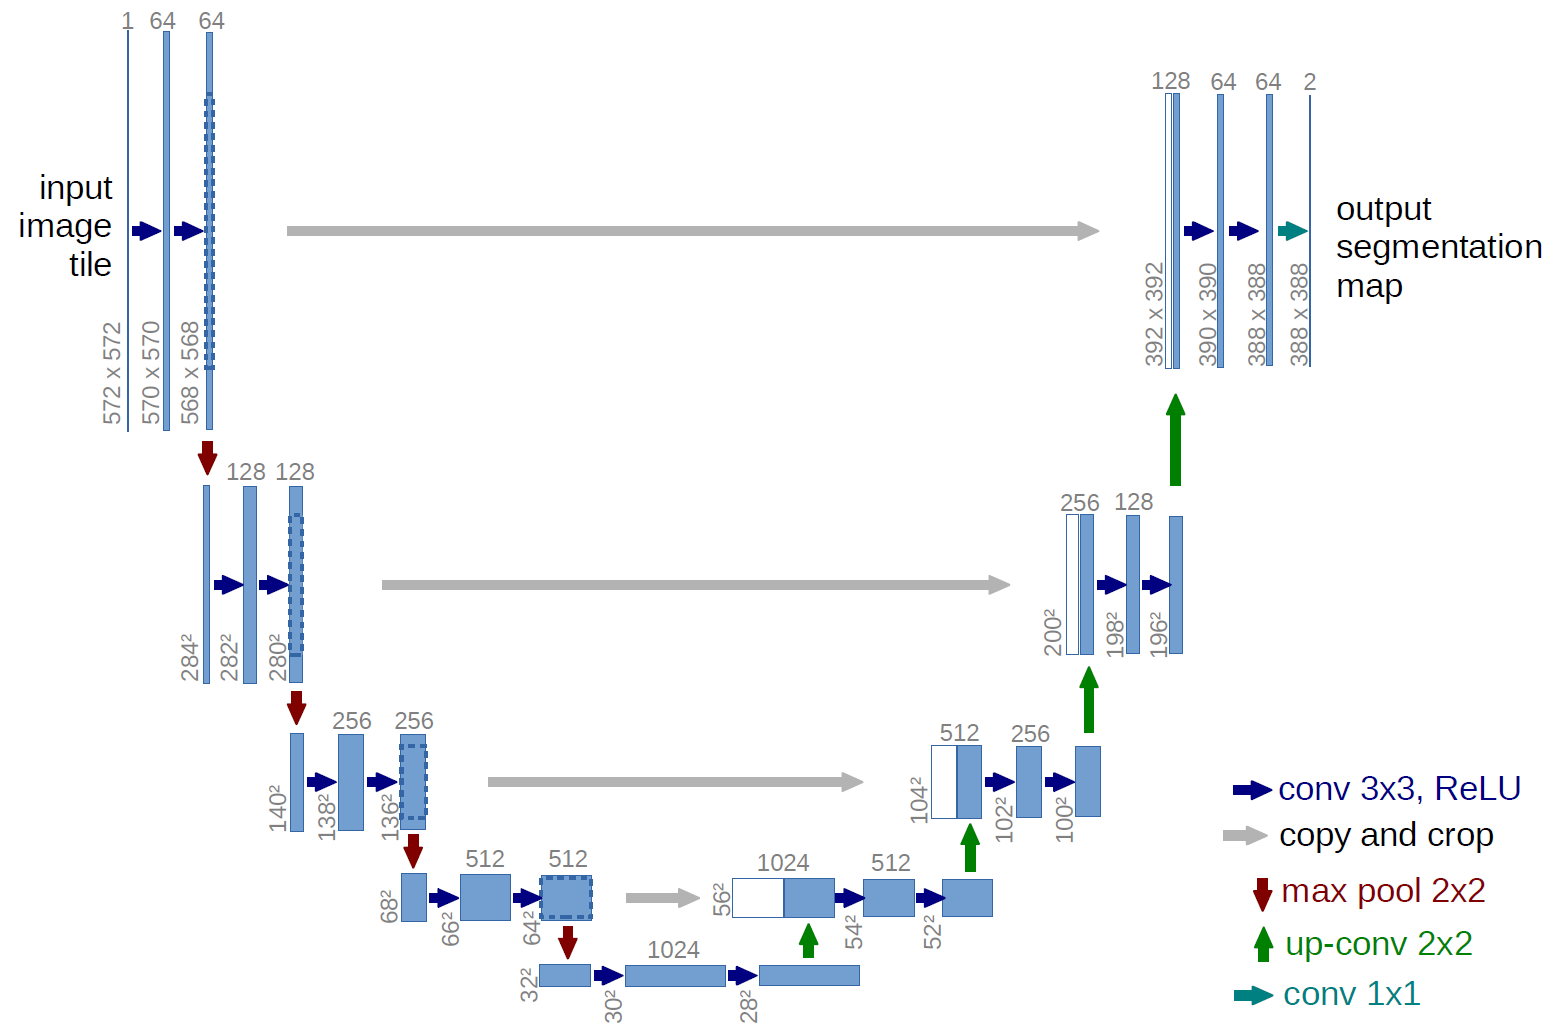
\includegraphics[width=\columnwidth]{../images/u-net-architecture.png}
\caption{U-Net Architecture. From \textsuperscript{\cite{ronneberger2015u}}}
\label{fig:CNN}
\end{figure}

\subsubsection{Performance}
The u-net is fast and precise model for segmentation of images. Up to now it has outperformed the prior best method (a sliding-window convolutional network) on the ISBI challenge for segmentation of neuronal structures in electron microscopic stacks. It has won the Grand Challenge for Computer-Automated Detection of Caries in Bitewing Radiography at ISBI 2015, and it has won the Cell Tracking Challenge at ISBI 2015 on the two most challenging transmitted light microscopy categories (Phase contrast and DIC microscopy) by a large margin.

\subsection{SegNet}

SegNet is a semantic segmentation model designed in 2017. This core trainable segmentation architecture consists of an encoder network, a corresponding decoder network followed by a pixel-wise classification layer. The architecture of the encoder network is topologically identical to the 13 convolutional layers in the VGG16 network. The role of the decoder network is to map the low resolution encoder feature maps to full input resolution feature maps for pixel-wise classification. The novelty of SegNet lies is in the manner in which the decoder upsamples its lower resolution input feature maps. Specifically, the decoder uses pooling indices computed in the max-pooling step of the corresponding encoder to perform non-linear upsampling. \textsuperscript{\cite{badrinarayanan2017segnet}}

\begin{figure}[h]
\centering
  \vspace{-0.1in}
    \centerline{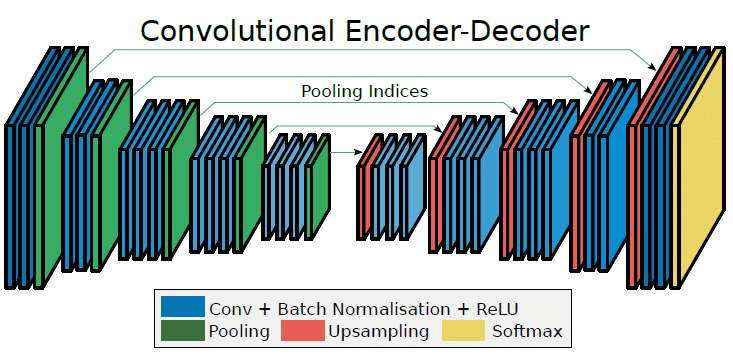
\includegraphics[width = 4in, height = 2.2in]{../images/segnet.png}}
    \caption{SegNet architecture}
\end{figure}

\section{Image Processing Methods}
\vspace{0.2in}
\hspace*{0.16in}

\subsection{Watershed}

Watershed segmentation is a region-based method that has its origins in mathematical morphology, The general concept was introduced by \textsuperscript{\cite{digabel1978iterative}}.
In watershed segmentation an image is regarded as a topographic landscape with ridges and valleys. The elevation values of the landscape are typically defined by the gray values of the respective pixels or their gradient magnitude. Based on such a 3D representation the watershed transform decomposes an image into catchment basins. For each local minimum, a catchment basin comprises all points whose path of steepest descent terminates at this minimum. Watersheds separate basins from each other. The watershed transform decomposes an image completely and thus assigns each pixel either to a region or a watershed. With noisy medical image data, a large number of small regions arises. This is known as the “over-segmentation” problem. \textsuperscript{\cite{Vincent_And_Soille_2022_sciencedirect}}

\begin{figure}[H]
\centering
\begin{minipage}{.33\textwidth}
  \centering
  \centerline{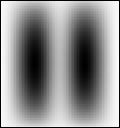
\includegraphics[width = 4in, height = 2.2in]{../images/watershed_example.jpg}}
    \subcaption{example Image}
\end{minipage}

\begin{minipage}{.33\textwidth}
  \centering
  \centerline{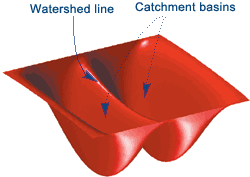
\includegraphics[width = 4in, height = 2.2in]{../images/watershed_relief.png}}
    \subcaption{watershed reliefs}
\end{minipage}
  \caption{Watershed algorithm from \textsuperscript{\cite{Steve_Eddins_2022_mathworks}}}
\end{figure}

\subsection{Connected Component Labeling}
Connected component labeling (also known as connected component analysis, blob extraction, or region labeling) is an algorithmic application of graph theory used to determine the connectivity of “blob”-like regions in a binary image.

When using contour analysis, we are often restricted by the hierarchy of the outlines (i.e., one contour contained within another). With connected component analysis, we can more easily segment and analyze these structures.

A great example of connected component Labeling is that we are using this algorith in cell counting, when we get the image mask we are using it to label all the non connected objects of the image, each object is labeled with a unique color as we can see in fig \ref{fig:connected_component_labeling}.

\begin{figure}[H]
\centering
\begin{minipage}{\textwidth}
  \centering
  \centerline{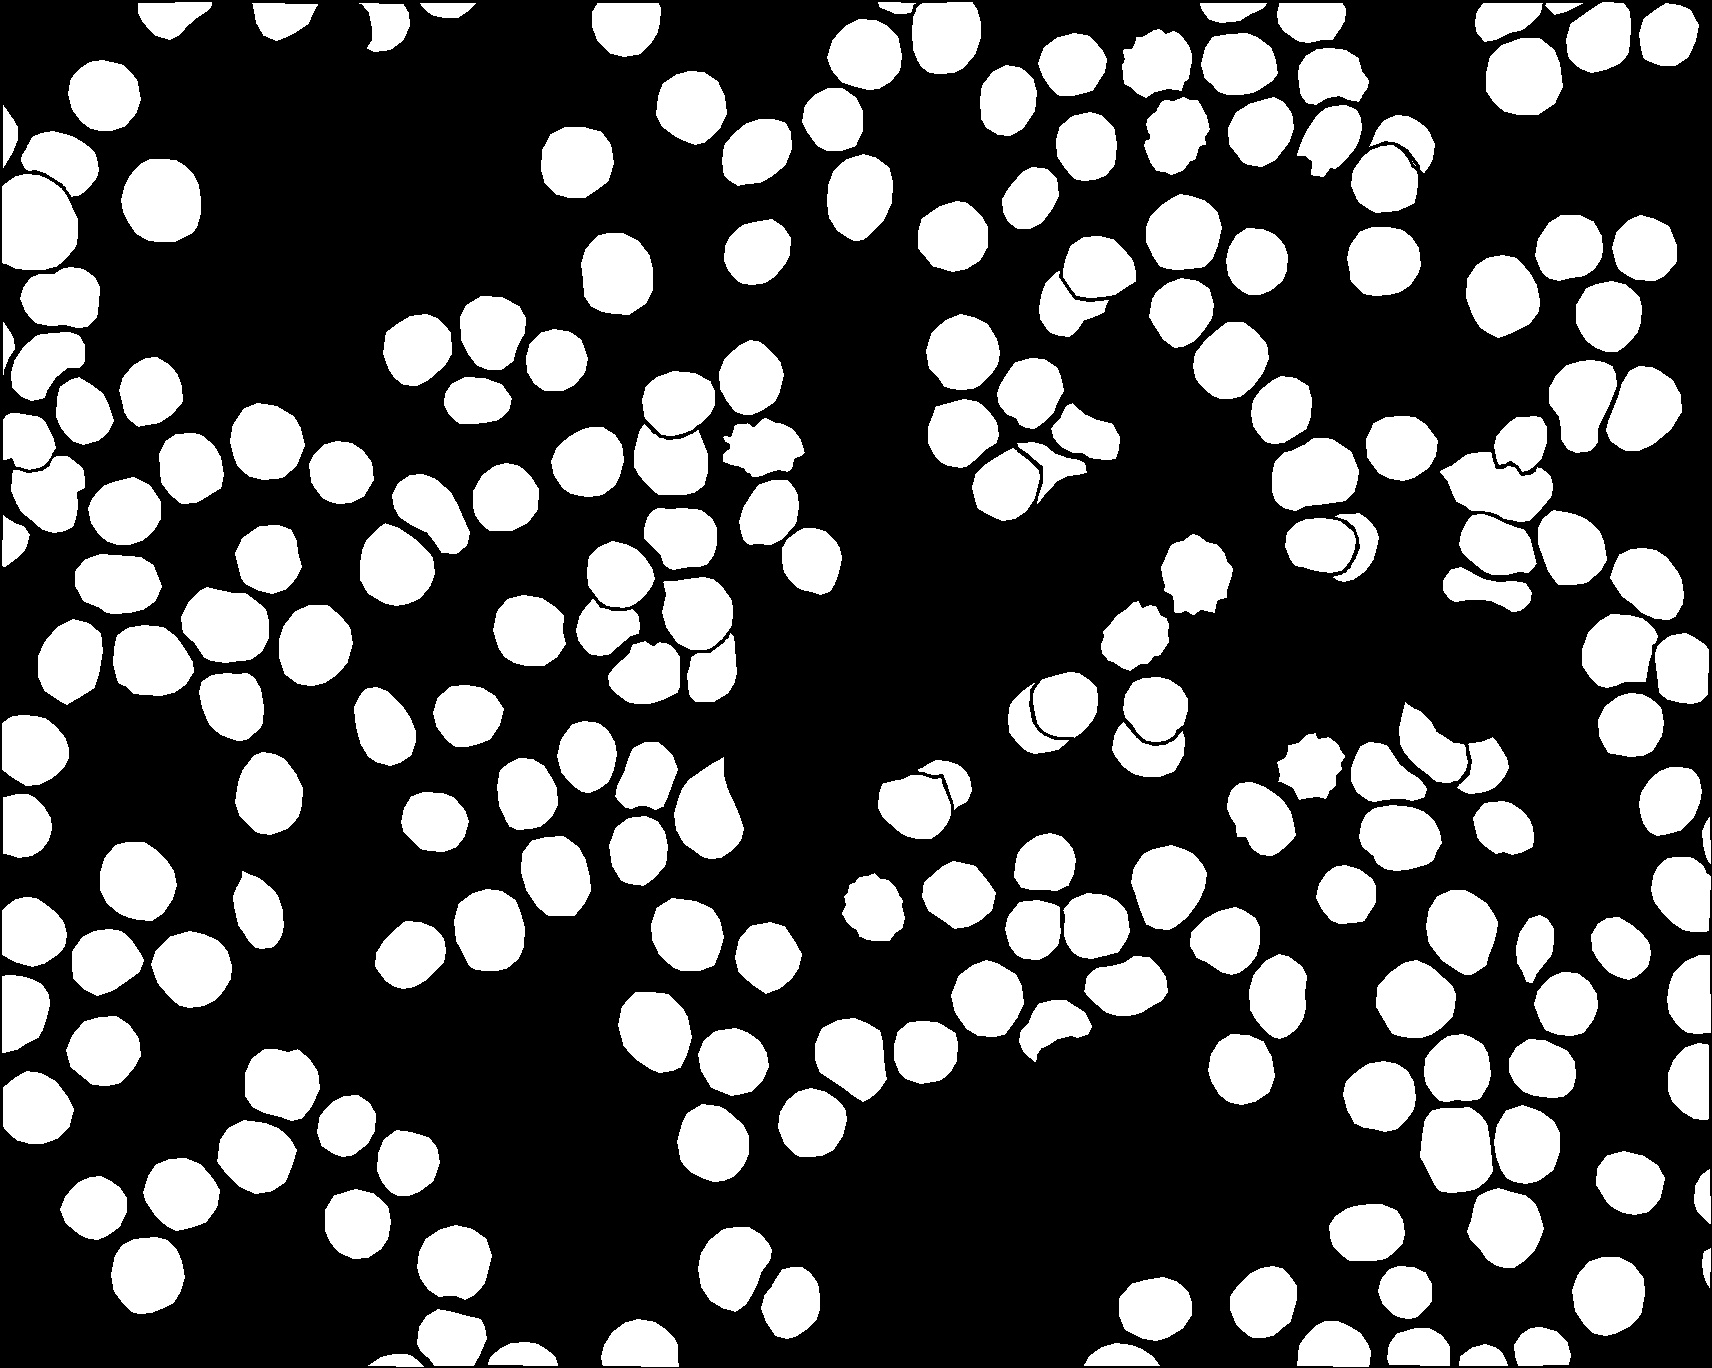
\includegraphics[width = 5in]{../images/Im0001_1_substraction.jpg}}
    \subcaption{example Image}
\end{minipage}

\begin{minipage}{\textwidth}
  \centering
  \centerline{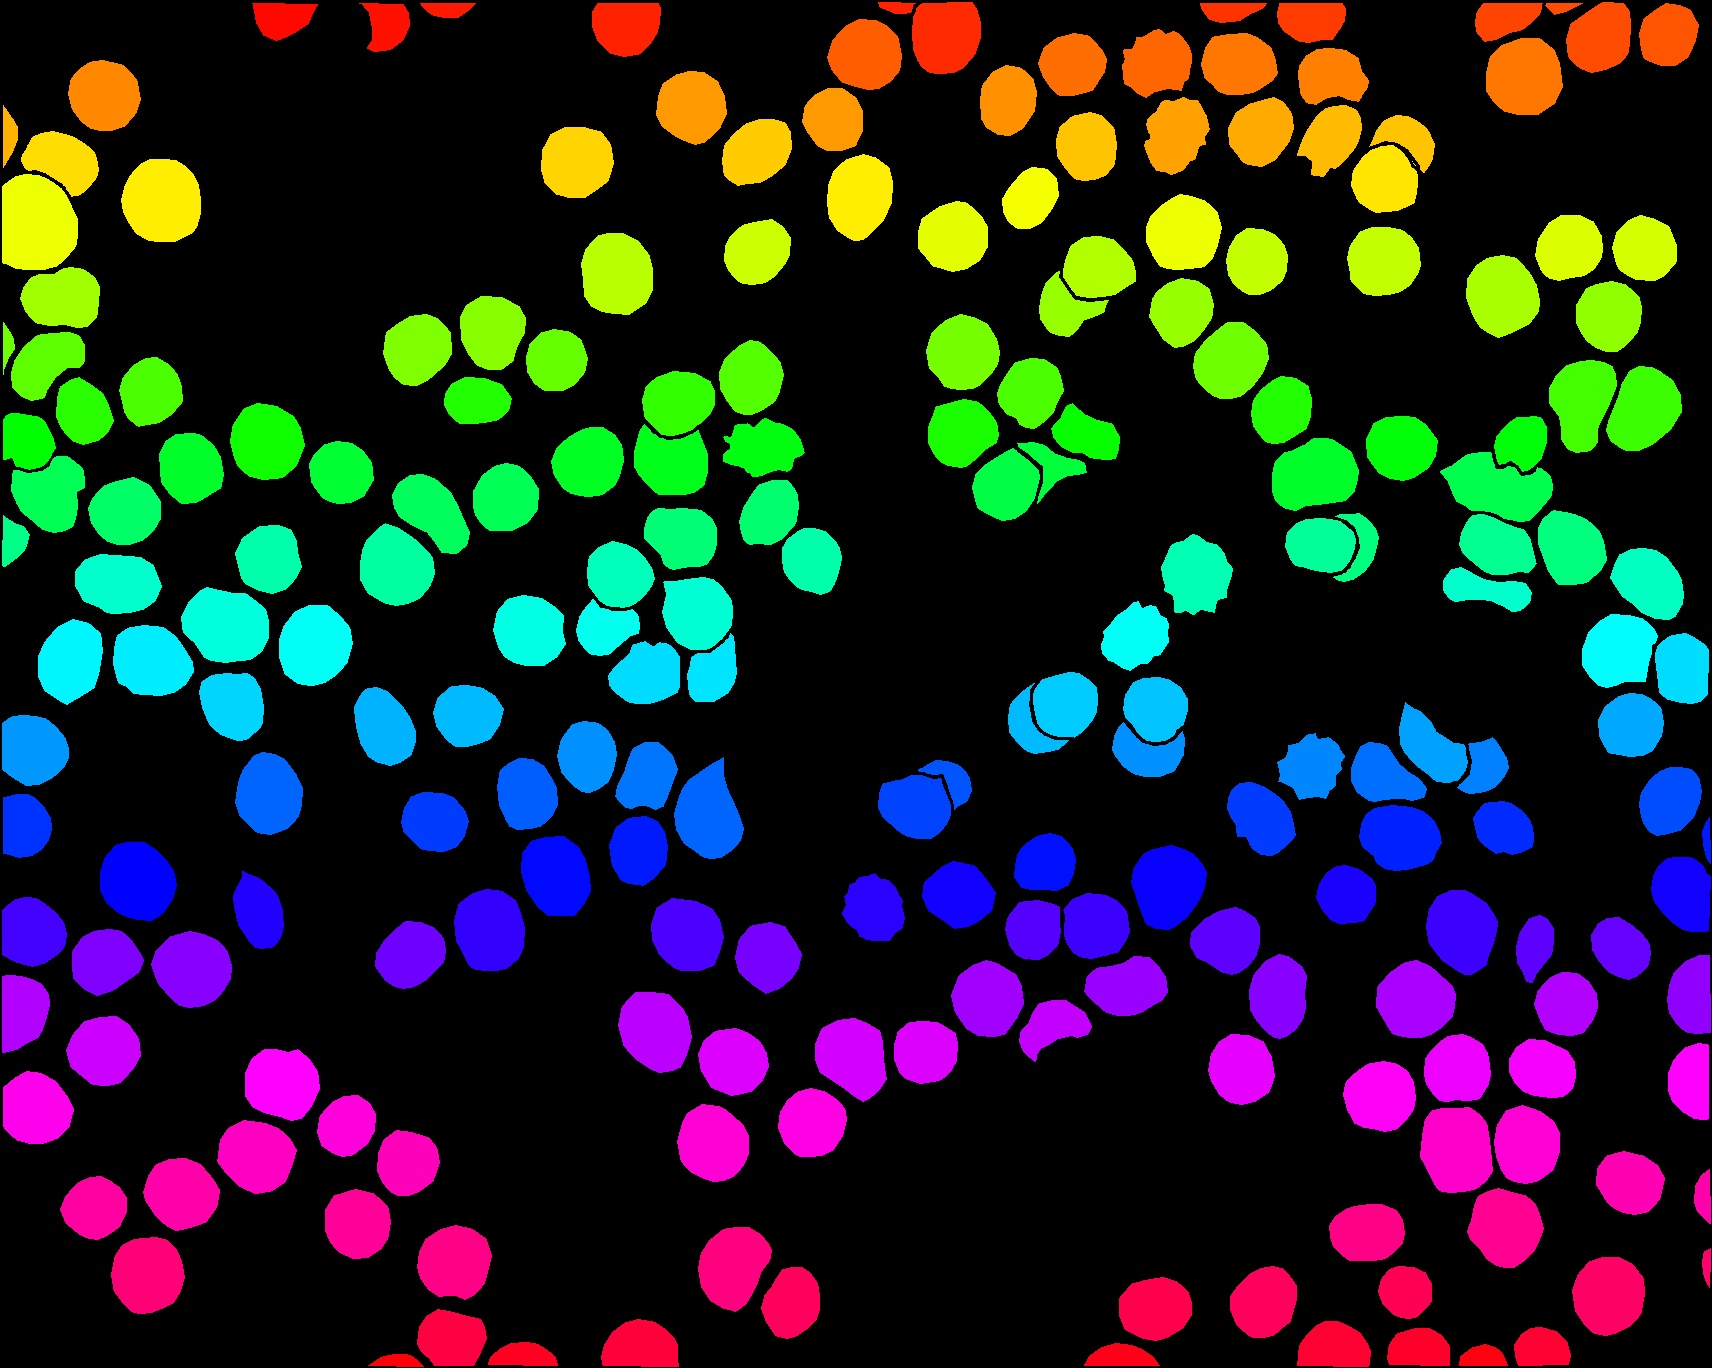
\includegraphics[width = 5in]{../images/Im0001_1_connected_compounent_labeling.jpg}}
    \subcaption{result image}
\end{minipage}
  \caption{Example of connected component labeling}
\end{figure}


\subsection{Discrete cosine transform}
A discrete cosine transform (DCT) expresses a finite sequence of data points in terms of a sum of cosine functions oscillating at different frequencies. The DCT, first proposed by Nasir Ahmed in 1972 \textsuperscript{\cite{ahmed1974discrete}}, is a widely used transformation technique in signal processing and data compression. It is used in most digital media, including digital images, digital video, digital audio, digital television, digital radio, and speech coding. DCTs are also important to numerous other applications in science and engineering, such as digital signal processing, telecommunication devices, reducing network bandwidth usage, and spectral methods for the numerical solution of partial differential equations.
the equation for the discrete cosine transform is represented as:

\begin{equation}
    c(u,v)=\alpha (u)\alpha (v)\sum_{u=0}^{N-1}\sum_{v=0}^{N-1} f(x,y) cos {\begin{bmatrix} {{\pi (2x + 1)u}\over{2N}} \end{bmatrix}} cos {\begin{bmatrix} {{\pi (2y + 1)v}\over{2N}} \end{bmatrix}} ,
    \label{eq:Discrete cosine transform equation}
\end{equation}

\begin{figure}[H]
\centering
    \centerline{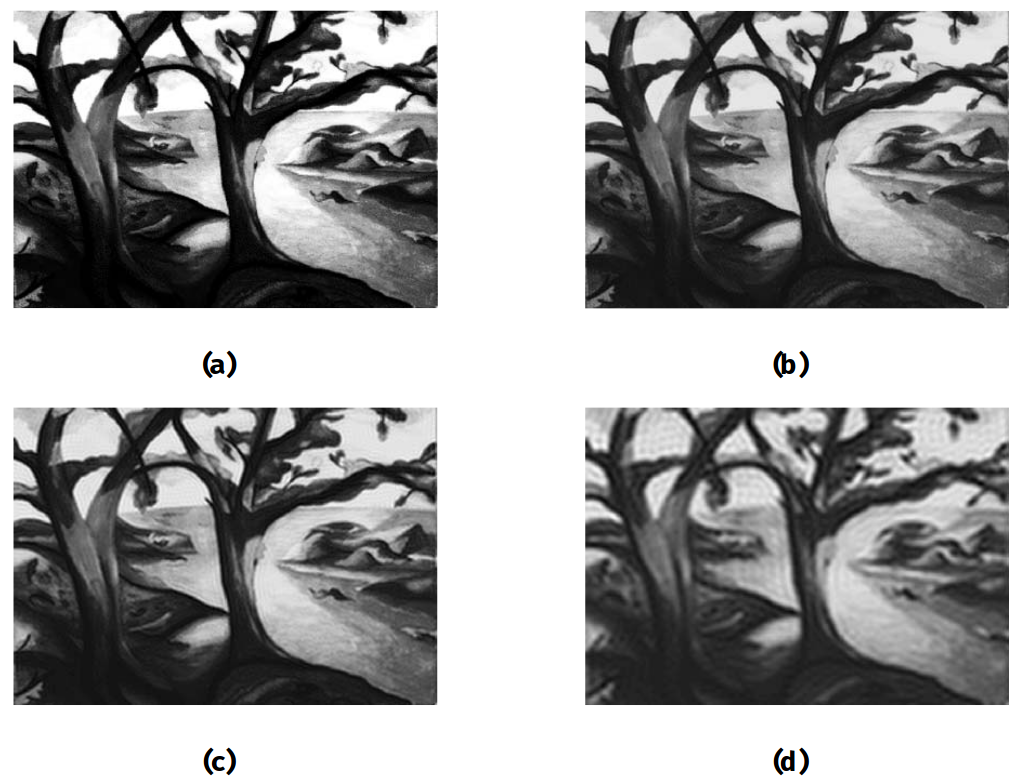
\includegraphics[width = 4.6in, height = 4.2in]{../images/inverse-DCT-of-trees.png}}
    \caption{Inverse DCT of Trees; (a) DCT(100\%); (b) DCT(75\%); (c) DCT(50\%); (d) DCT(25\%).}
\end{figure}

\subsection{Circular Hough Transform}

The general Hough transform can be used on any kind of shape, although the complexity of the transformation increase with the number of parameters needed to describing the shape. \textsuperscript{\cite{pedersen2007circular}}
The circle Hough Transform (CHT) is a basic feature extraction technique used in digital image processing for detecting circles in imperfect images.

In a two-dimensional space, a circle can be described by:

\begin{equation}
    (x - a)^2 + (y - b)^2 = r^2
\end{equation}

where (a,b) is the center of the circle, and r is the radius. If a 2D point (x,y) is fixed, then the parameters can be found according to (1). The parameter space would be three dimensional, (a, b, r). And all the parameters that satisfy (x, y) would lie on the surface of an inverted right-angled cone whose apex is at (x, y, 0). In the 3D space, the circle parameters can be identified by the intersection of many conic surfaces that are defined by points on the 2D circle. This process can be divided into two stages. The first stage is fixing radius then find the optimal center of circles in a 2D parameter space. The second stage is to find the optimal radius in a one dimensional parameter space.

This is the Circular Hough Transform algorithm:

\begin{enumerate}
    \item For each A[a,b,r] = 0;
    \item Process the filtering algorithm on image Gaussian Blurring, convert the image to grayscale ( grayScaling), make Canny operator, The Canny operator gives the edges on image.
    \item Vote the all possible circles in accumulator.
    \item The local maximum voted circles of Accumulator A gives the circle Hough space.
    \item The maximum voted circle of Accumulator gives the circle. \textsuperscript{\cite{circle-hough-transform}}
\end{enumerate}

\subsection{Distance Transform}

A Distance Transform, also known as distance map or distance field, is a derived representation of a digital image. The choice of the term depends on the point of view on the object in question: whether the initial image is transformed into another representation, or it is simply endowed with an additional map or field.

Distance fields can also be signed, in the case where it is important to distinguish whether the point is inside or outside of the shape. \textsuperscript{\cite{frisken2000adaptively}}

The map labels each pixel of the image with the distance to the nearest obstacle pixel. A most common type of obstacle pixel is a boundary pixel in a binary image.

\subsection{Marching Squares Algorithm}

Marching squares is a computer graphics algorithm that generates contours for a two-dimensional scalar field (rectangular array of individual numerical values). A similar method can be used to contour 2D triangle meshes.

The contours can be of two kinds:

\begin{itemize}
    \item Isolines – lines following a single data level, or isovalue.
    \item Isobands – filled areas between isolines.
\end{itemize}

Typical applications include the contour lines on topographic maps or the generation of isobars for weather maps.

Marching squares takes a similar approach to the 3D marching cubes algorithm:

\begin{itemize}
    \item Process each cell in the grid independently.
    \item Calculate a cell index using comparisons of the contour level(s) with the data values at the cell corners.
    \item Use a pre-built lookup table, keyed on the cell index, to describe the output geometry for the cell.
    \item Apply linear interpolation along the boundaries of the cell to calculate the exact contour position. \textsuperscript{\cite{maple2003geometric}}
\end{itemize}


\newpage
